\documentclass[12pt, a4paper]{article}
\usepackage[top=1.0in, bottom=1.0in, left=0.8in, right=0.8in]{geometry}

\setlength{\parskip}{\baselineskip}%
\setlength{\parindent}{0pt}%
\usepackage{bookmark}
\usepackage[]{graphicx}
\usepackage{enumitem}
\usepackage{amsmath}
\usepackage{relsize}
\usepackage{cprotect}
\usepackage{amsmath, amsfonts}
\usepackage{siunitx}
\usepackage{mathrsfs}
\usepackage{framed}
\usepackage{enumitem}
\usepackage{tikz}
\usepackage{circuitikz}
\usepackage{float}
\usepackage[english]{babel}
\usepackage{blindtext}

\newlist{notes}{enumerate}{1}
\setlist[notes]{label=\textbf{Note:} ,leftmargin=*}

\newlist{hints}{enumerate}{1}
\setlist[hints]{label=\textbf{Hint:} ,leftmargin=*}

\usepackage{xcolor}
\usepackage{color}
\definecolor{com1}{RGB}{125,125,125}
\definecolor{comment}{RGB}{140,115,115}
\definecolor{numbering}{rgb}{0.2,0.2,0.2}
\definecolor{key}{RGB}{0,0,180}
\definecolor{in}{RGB}{0,100,0}
\definecolor{out}{RGB}{100,30,30}
\definecolor{bg}{RGB}{245,245,245}
\definecolor{bgLight}{RGB}{250,250,250}
\definecolor{string}{RGB}{0,150,0}

\usepackage{hyperref}
\hypersetup{
    colorlinks=true,
    linkcolor=blue,
    filecolor=magenta,      
    urlcolor=blue,
}
\urlstyle{same}

\usepackage{listings}

\lstdefinestyle{py_code}{ %
    backgroundcolor=\color{bg},      % choose the background
    basicstyle=\ttfamily\small,		      % fonts
    breakatwhitespace=false,         % automatic breaks at whitespace ?
    breaklines=true,                 % sets automatic line breaking
    captionpos=b,                    % caption-position - bottom
    commentstyle=\itshape\color{comment},    % comment style
    extendedchars=true,              % use non-ASCII
    frame=single,	                   % single frame around the code
    keepspaces=true,                 % keeps spaces in text
    keywordstyle=\bfseries\color{key},% keyword style
    language=Python,                 	  % the language of the code
    morekeywords={Null},       % add more keywords to the set
    numbers=left,                    % line_numbers (none, left, right)
    numbersep=10pt,                  % line_no - code dist
    numberstyle=\footnotesize\color{numbering}, % line_no style
    rulecolor=\color{black},         % frame_color [!always set]
    showspaces=false,                % show spaces everywhere
    showstringspaces=false,          % 
    showtabs=false,                  % 
    stepnumber=1,                    % step b/w two line-no
    stringstyle=\color{string},     % string literal style
    tabsize=2,	                       % sets default tabsize to 2 spaces
    title=\lstname,                  % show the filename
    escapeinside={(*}{*)},			  % escape from style inside (* *)
    xleftmargin=\parindent,
    belowskip=-1.3 \baselineskip,
    aboveskip=1.0 \baselineskip,
    columns=fullflexible,
    xleftmargin=0.15in,
}
\lstnewenvironment{py_code}
{\lstset{style=py_code}}
{}

\lstdefinestyle{psudo}{ %
    backgroundcolor=\color{bgLight},   % choose the background
    basicstyle=\ttfamily\small,		      % fonts
    breakatwhitespace=false,         % automatic breaks at whitespace ?
    breaklines=true,                 % sets automatic line breaking
    captionpos=b,                    % caption-position - bottom
    commentstyle=\itshape\color{com1},          % comment style
    extendedchars=true,              % use non-ASCII
    keepspaces=true,                 % keeps spaces in text
    language=C,                 	  % the language of the code
    morekeywords={type,NULL, True, False},       % add more keywords to the set
    showspaces=false,                % show spaces everywhere
    showstringspaces=false,          % 
    showtabs=false,                  % 
    tabsize=2,	                       % sets default tabsize to 2 spaces
    title=\lstname,                  % show the filename
    escapeinside={(*}{*)},			  % escape from style inside (* *)
    belowskip=-1.8 \baselineskip,
    aboveskip=0.9 \baselineskip,
    columns=fullflexible,
    xleftmargin=0.2in,
    frame=tb,
    framexleftmargin=16pt,
    framextopmargin=6pt,
    framexbottommargin=6pt, 
    framerule=0pt,
}

\lstnewenvironment{psudo}
{\lstset{style=psudo}}
{}

\graphicspath{ ./ }

\title{\textbf{EE2703 : Applied Programming Lab \\ Assignment 7 \\ Circuit Analysis using Sympy}} 
\author{Chagari Koushal Kumar Reddy \\ EE20B023} % Author name

\date{\today} % Date for the report

\begin{document}		

\maketitle % Insert the title, author and date
\clearpage

\tableofcontents
\clearpage

\section{Aim}
The aim to this assignment is to:
\begin{enumerate}
    \item Get started with some basic Sympy (Symbolic python) commands
    \item Solve for the output response of given active Low pass and High pass filters using Sympy and Scipy.signal toolbox
    \item Analyze the frequency components in output responses
\end{enumerate}
\section{Theory: Active RC Filters}
Active RC filters are electronic devices which are purely made using active operational amplifiers (OpAmps), resistors and capacitors.
These filters help us to filter out certain frequency components present in an electric signal which may not be desirable for particular application.
They are used in various applications such as noise reduction, radio tuning, selective amplification etc. In this assignment, two types of active RC filters are analyzed: Butterworth Low Pass Filter and Butterworth High Pass Filter.
\subsection{Butterworth Low Pass Filter}
A Low Pass Filter (LPF) is an electrical filter which allows only the low frequency components of an electric signal and attenuates the high frequency components. The electronic used to realize a Butterworth LPF is shown below:
\vspace*{-0.5cm}
\begin{figure}[H]
    \centering
    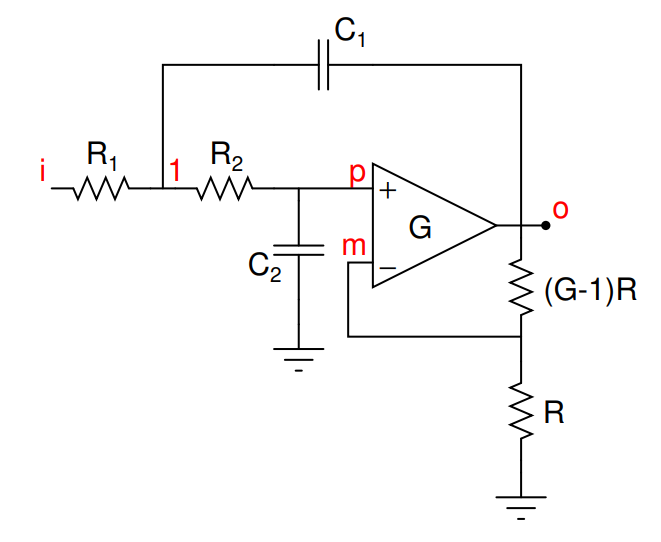
\includegraphics[scale = 0.8]{Figure_blpf.png}
    \label{fig:sample}
\end{figure}
We need to solve for the transfer function $H(s)=\frac{V_{o}(s)}{V_{i}(s)}$. To do this, we need to solve for the node voltages using nodal analysis. Also, we know that in the laplace domain, a capacitor acts like resistor with its resistance as $R=\frac{1}{sC}$.
With these things in mind, the nodal equations in matrix form are given by:
\begin{equation*}
\begin{bmatrix}
    0 & 0 & 1 & \frac{-1}{G}\\
    -\frac{1}{1+sR_{2}C_{2}} & 1 & 0 & 0\\
    0 & -G & G & 1\\
    -\frac{1}{R_{1}}-\frac{1}{R_{2}}-sC_{1} & \frac{1}{R_{2}} & 0 & sC_{1}
\end{bmatrix}
\begin{bmatrix}
    V_{1}\\
    V_{p}\\
    V_{m}\\
    V_{o}
\end{bmatrix}
=
\begin{bmatrix}
    0\\
    0\\
    0\\
    -\frac{V_{i}(s)}{R_{1}}
\end{bmatrix}
\end{equation*}
Clearly the source vector on the RHS contains only one non-zero term dependent on $V_{i}$. Hence all the other node voltages would be some multiple fo it. We need the multiple relating $V_{o}$ and that multiple is the transfer function $H(s)$.
\subsection{Butterworth High Pass Filter}
A high pass filter (HPF) is an electrical filter which allows only the high frequency components of an electric signal and attenuates the low frequency components. The electronic circuit used to realise a Butterworth HPF is shown below:
\vspace*{-0.5cm}
\begin{figure}[H]
    \centering
    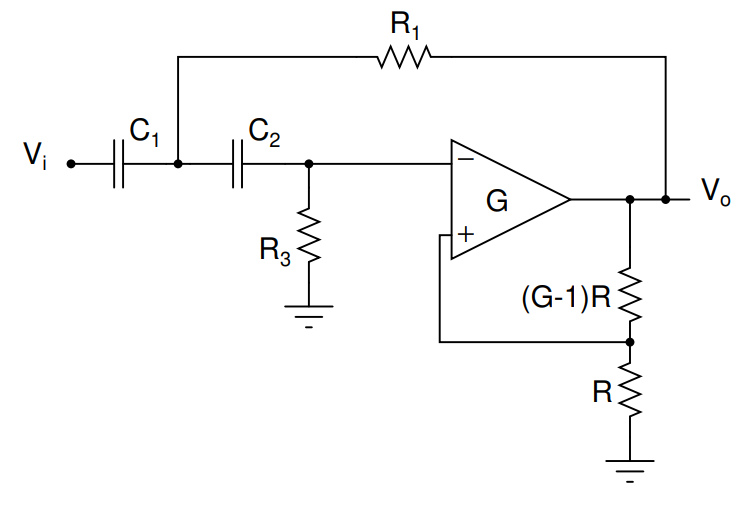
\includegraphics[scale = 0.8]{Figure_bhpf.png}
    \label{fig:sample}
\end{figure}
The circuit is almost similar to the LPF circuit except that the resistors are replaced by capacitors and vice-versa (Except for feedback resistors). Also, there isn't much change in the structure of the nodal matrix equation. With the understanding that whatever was initially a resistor is now replaced by a capacitor and vice-versa, we can apply the following transform:
\begin{equation*}
    R \rightarrow \frac{1}{sC}
\end{equation*}
\begin{equation*}
    sC \rightarrow \frac{1}{R}
\end{equation*}
With these changes in mind, the new matrix equation becomes:
\begin{equation*}
    \begin{bmatrix}
        0 & 0 & 1 & \frac{-1}{G}\\
        -\frac{sC_{2}R_{3}}{1+sC_{2}R_{3}} & 1 & 0 & 0\\
        0 & -G & G & 1\\
        -\frac{1}{R_{1}}-sC_{1}-sC_{2} & sC_{2} & 0 & \frac{1}{R_{1}}
    \end{bmatrix}
    \begin{bmatrix}
        V_{1}\\
        V_{p}\\
        V_{m}\\
        V_{o}
    \end{bmatrix}
    =
    \begin{bmatrix}
        0\\
        0\\
        0\\
        -sC_{1}V_{i}(s)
    \end{bmatrix}
\end{equation*}
Again the output response $V_{o}$ will be some multiple of $V_{i}$ and that multiple is the HPF transfer function $H(s)$.
\subsection{Solving for the transfer function}
As we have seen, the matrix equation is not purely based on numbers. It is also
based on mathematical variables. In our case, the variable is 's'. Unlike normal
matrix equations, we can't solve this using packages such as numpy. We need to
treat the variable 's' as an unknown entity and solve for the transfer function as
a function of 's'. To do this, we need the Sympy library of python. Sympy is a
special library which allows us to treat certain variables as mathematical/sym-
bolic variables. These variables are different from the usual python variables.
They necessarily need not store values but rather store symbols. These sym-
bols don't have any value but can be treated like the variables we use in math
(x,y,z) and complex expressions could be formed using these symbols. Finally
the value of that expression can be found by providing these symbols some
numerical values.

Sympy is very useful when it comes to obtain the expression from primitive
inputs. In our filter case too, the primitive inputs are the resistor and capacitor
values. However, the final expression is not easily derivable and hence, we
can't write a user-defined python function without knowing the final expression.
Sympy allows us to find the final expression while still treating the variable 's'
as a mathematical variable.
\begin{py_code}
    import sympy as sp
    s = sp.symbols('s')

    def lowpass(R1,R2,C1,C2,G,Vi):
        A = sp.Matrix([ [0,0,1,-1/G], [-1/(1+s*R2*C2),1,0,0], [0,-G,G,1], [-(1/R1)-(1/R2)-s*C1,1/R2,0,s*C1]])
        b = sp.Matrix([0,0,0,-Vi/R1])
        V = A.inv()*b
        Vo = V[3]
        return Vo
\end{py_code}
For example, in the python function provided above, the inputs are the resistor,
capacitor and Opamp gain values. However, the final expression is not directly
used to find the transfer function. Instead, the sympy variable ’s’ is used to
denote the variable and the matrix equation is solved. Finally, the expression
is obtained and returned out.
\section{Functions defined in Code}
\subsection{Function to generate the LPF transfer function}
The following function returns the transfer function of the LPF.
\begin{py_code}
    def lowpass(R1,R2,C1,C2,G,Vi):
        A = sp.Matrix([ [0,0,1,-1/G], [-1/(1+s*R2*C2),1,0,0], [0,-G,G,1], [-(1/R1)-(1/R2)-s*C1,1/R2,0,s*C1]])
        b = sp.Matrix([0,0,0,-Vi/R1])
        V = A.inv()*b
        Vo = V[3]
        return Vo
\end{py_code}
\subsection{Function to generate the HPF transfer function}
The following function returns the transfer function of the HPF.
\begin{py_code}
    def highpass(R1,R3,C1,C2,G,Vi):
        A = sp.Matrix([ [0,0,1,-1/G], [-s*C2,(1/R3)+s*C2,0,0], [0,-G,G,1], [s*C1+s*C2+(1/R1),-s*C2,0,-1/R1]])
        b = sp.Matrix([0,0,0,Vi*s*C1])
        V = A.inv()*b
        Vo = V[3]
        return Vo
\end{py_code}
\subsection{Function to convert transfer function expression to LTI form of signal toolbox}
This function takes a transfer function expression as input, converts it to the signal toolbox LTI form and returns it.
\begin{py_code}
    def sympy_tf2sig_tf(tf):
        n,d = tf.as_numer_denom()
        num = n.as_poly(s).all_coeffs()
        den = d.as_poly(s).all_coeffs()
        num = [float(i) for i in num]
        den = [float(i) for i in den]
        TF = sig.lti(num,den)
        return TF
\end{py_code}
\subsection{Function to generate damped sinusoid responses}
This function takes the transfer function, damping factor, frequency and time as the inputs. It computes the response and returns it.
\begin{py_code}
    def damped_sinusoid_response(H,A,B,t):
        V_in = np.exp(-A*t)*np.cos(B*t)
        V_o = sig.lsim(H,V_in,t)[1]
        return V_o
\end{py_code}
\section{Observations and Plots}
\subsection{Magnitude Response Plots}
\vspace*{-0.5cm}
\begin{figure}[H]
    \centering
    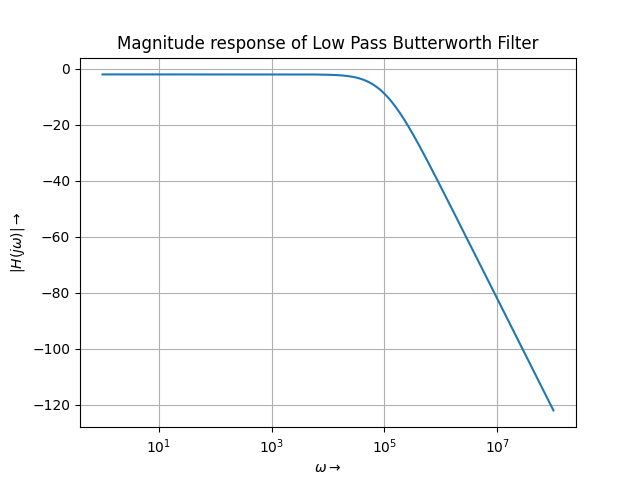
\includegraphics[scale = 0.8]{Figure_1.png}
    \label{fig:sample}
\end{figure}
\begin{center}
    The LPF seems to have a single pole at frequency = $10^{5}$ rad/s
\end{center}
\vspace*{-1.5cm}
\begin{figure}[H]
    \centering
    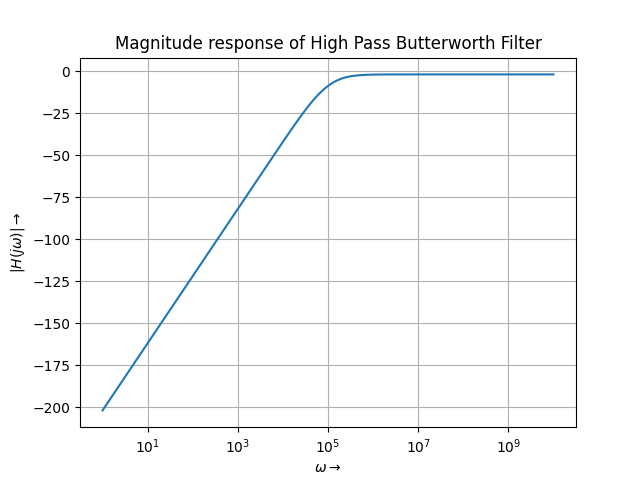
\includegraphics[scale = 0.8]{Figure_4.png}
    \label{fig:sample}
\end{figure}
\begin{center}
    The HPF seems to have DC zero and a single pole at frequency = $10^{5}$ rad/s
\end{center}
\subsection{Step Response Plots}
\vspace*{-0.5cm}
\begin{figure}[H]
    \centering
    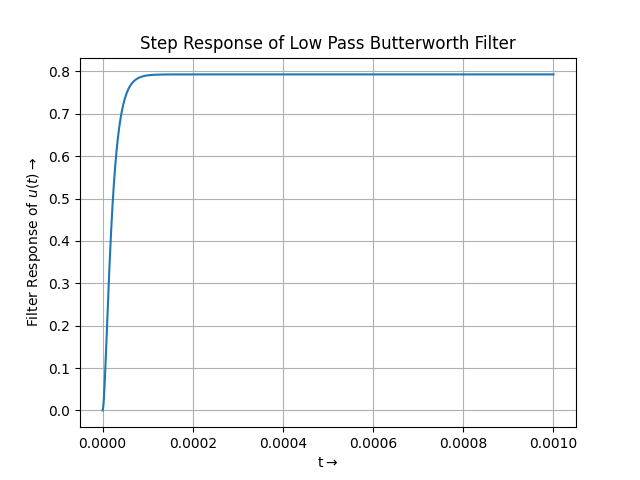
\includegraphics[scale = 0.8]{Figure_2.png}
    \label{fig:sample}
\end{figure}
\begin{center}
    The DC gain of the LPF is $\frac{G}{2} = 0.793$. Hence the step response is looking a like a DC signal after some time
\end{center}
\vspace*{-0.5cm}
\begin{figure}[H]
    \centering
    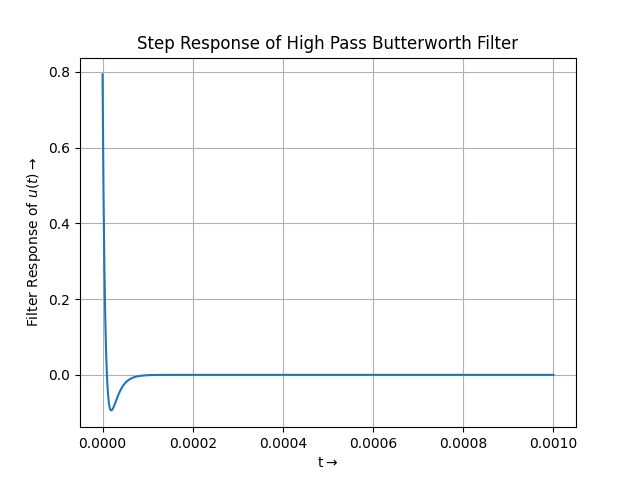
\includegraphics[scale = 0.8]{Figure_5.png}
    \label{fig:sample}
\end{figure}
\begin{center}
    The step response of HPF is a DC signal with value close to 0. The initial values cause the transient behaviour.
\end{center}

In this question we are asked whether we understood the response

The reason for the initial peak is the initial conditions. The capacitor does not allow instantaneous changes in the voltage across it. Before t = 0, both capacitors have no charge, and the
voltage across both is 0, and this will not change instantaneously.

Referring to the circuit diagram, the instant the 1V of the unit step is applied ($t=0^{+}$), the drop across the capacitors $C_{1}$ and $C_{2}$ will still be zero. Therefore $V_{m}=1V$.

$V_{m}=\frac{V_{o}}{G}$ and $V_{o}=G(V_{p}-V_{m})$, therefore we get:
\begin{equation*}
    V_{o} = G(1-\frac{V_{o}}{G})
\end{equation*}
\begin{equation*}
    V_{o} = \frac{G}{2} = \frac{1.586}{2} = 0.793V \approx 0.8V
\end{equation*}
And hence, we have an inital peaking around 0.8V and then it quickly decays and settles down to the expected 0V since it is a high pass filter and DC output should be 0V.
\subsection{Sum of Sinusoids Response Plots}
\vspace*{-0.5cm}
\begin{figure}[H]
    \centering
    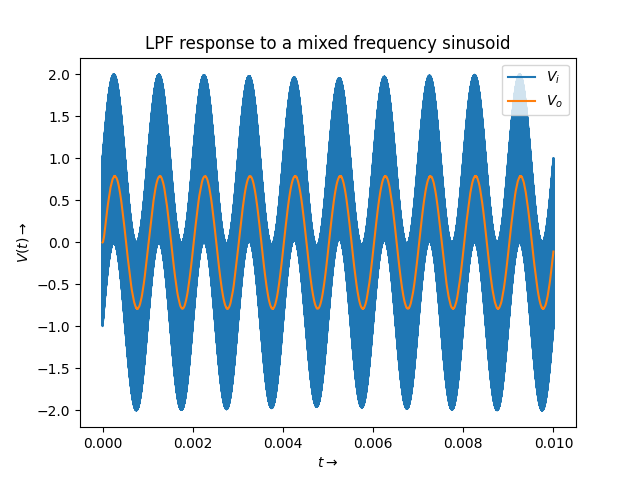
\includegraphics[scale = 0.8]{Figure_3.png}
    \label{fig:sample}
\end{figure}
\begin{center}
    The output response of the sum of sinusoids, when passed through an LPF purely contains only the f = 1kHz component 
\end{center}
\vspace*{-0.5cm}
\begin{figure}[H]
    \centering
    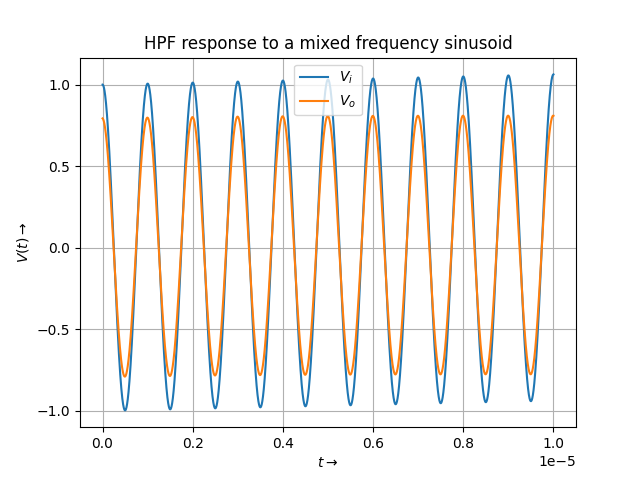
\includegraphics[scale = 0.8]{Figure_6.png}
    \label{fig:sample}
\end{figure}
\begin{center}
    The output response of the sum of sinusoids, when passed through HPF purely contains only the f = 1MHz component
\end{center}
\subsection{Damped Sinusoid Signals}
\vspace*{-0.5cm}
\begin{figure}[H]
    \centering
    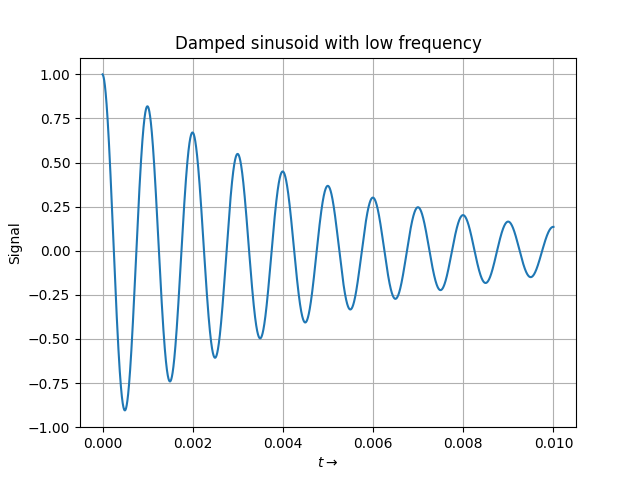
\includegraphics[scale = 0.8]{Figure_11.png}
    \label{fig:sample}
\end{figure}
\begin{center}
    This is a damped sinusoid signal with f = 1kHz and decay constant = 200$s^{-1}$
\end{center}
\vspace*{-0.5cm}
\begin{figure}[H]
    \centering
    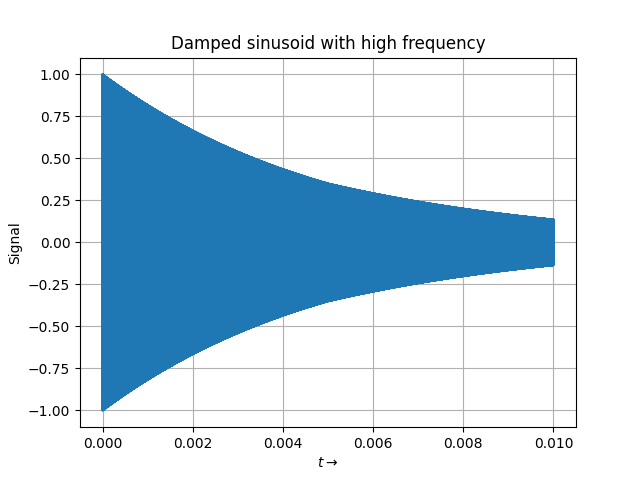
\includegraphics[scale = 0.8]{Figure_12.png}
    \label{fig:sample}
\end{figure}
\begin{center}
    This is a damped sinusoid signal with f = 1MHz and decay constant = 200$s^{-1}$
\end{center}
\subsection{Damped Sinusoid Signal Response Plots}
\vspace*{-0.5cm}
\begin{figure}[H]
    \centering
    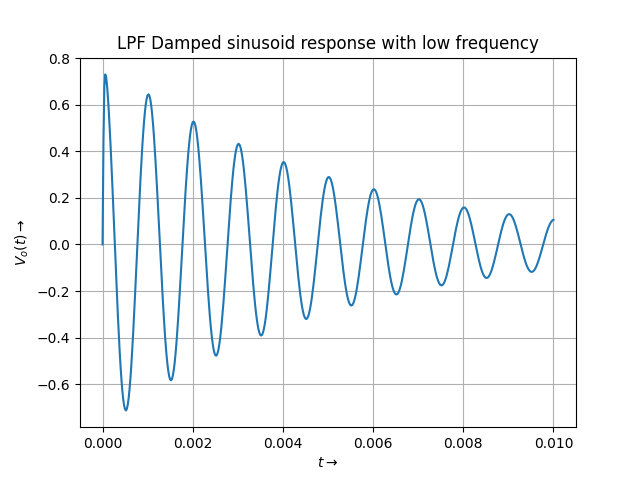
\includegraphics[scale = 0.8]{Figure_7.png}
    \label{fig:sample}
\end{figure}
\begin{center}
    When the low frequency damped sinusoid is passed through an LPF, the output isn't much different from the input. The amplitude has reduced to 0.793
\end{center}
\vspace*{-0.5cm}
\begin{figure}[H]
    \centering
    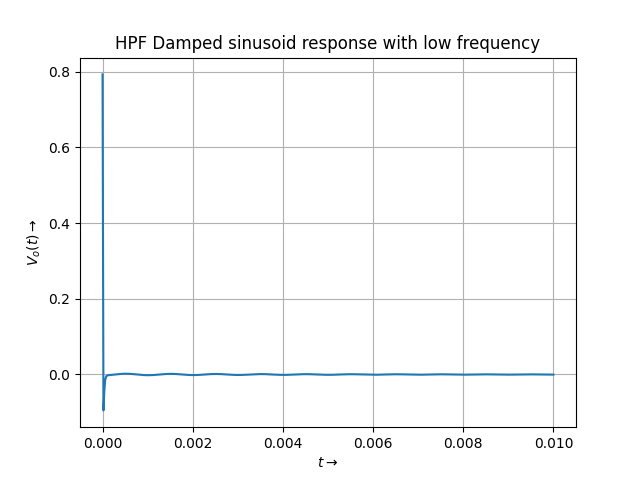
\includegraphics[scale = 0.8]{Figure_8.png}
    \label{fig:sample}
\end{figure}
\begin{center}
    When the low frequency damped sinusoid is passed through a HPF, the output is highly attenuated as seen from the image. The line at t=0 is due to inital conditions
\end{center}
\vspace*{-0.5cm}
\begin{figure}[H]
    \centering
    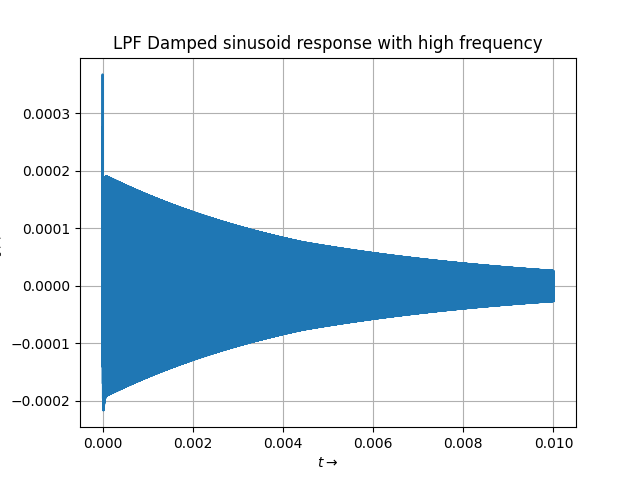
\includegraphics[scale = 0.8]{Figure_9.png}
    \label{fig:sample}
\end{figure}
\begin{center}
    When the high frequency damped sinusoid is passed through an LPF, the output is highly attenuated as seen from the image(Y-axis scale is very low)
\end{center}
\vspace*{-0.5cm}
\begin{figure}[H]
    \centering
    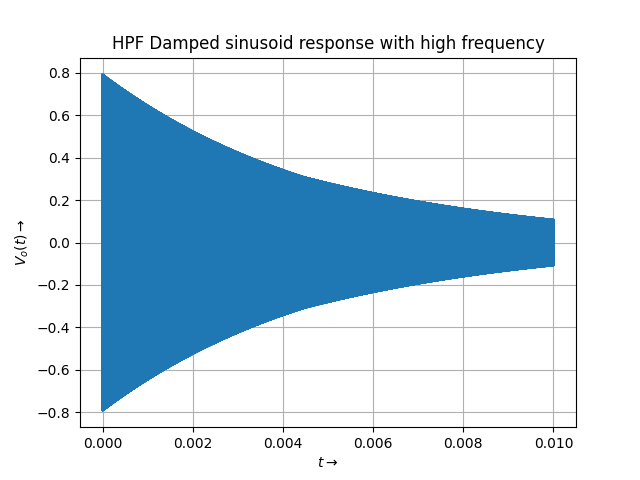
\includegraphics[scale = 0.8]{Figure_10.png}
    \label{fig:sample}
\end{figure}
\begin{center}
    When high frequency damped sinusoid is passed through a HPF, the output isn't much different from the input. The amplitude has reduced to 0.8
\end{center}
\section{Conclusions}
\begin{enumerate}
    \item Both the filters have a pole frequency of $10^{5}$ rad/s and a constant gain of 0.8 in their operating region. This is evident from their magnitude response plots.
    \item The step response of the low pass filter starts from zero (due to inital conditions) and stabilises at a DC value of 0.8
    \item The step response of the high pass filter starts from 0.8 (due to inital conditions) and stabilises to 0.
    \item When the sum of sinusoids signal is passed through the LPF, the 1kHz component gets filtered out with a gain of 0.8.
    \item When the sum of sinusoids signal is passed through the HPF, the 1MHz component gets filtered out with a gain of 0.8.
    \item When the low frequency damped sinusoid is passed through the LPF, the output is not so much different from the input.
    \item When the low frequency damped sinusoid is passed through the HPF, the output is highly attenuated. It starts from 0.8 due to inital conditions.
    \item When the high frequency damped sinusoid is passed through the LPF, the output is highly attenuated (Evident from the Y-Axis scale)
    \item When the high frequency damped sinusoid is passed through the HPF, the output is not so much different from the input.
\end{enumerate}
\end{document}